\graphicspath{{./lab03/Images/}}


\maketitlepage{App Development}{in Android Studio}{Lab 3: Components}
\maketocpage


\section{Activities}
We have already used an activity without going into too much detail what it is. An activity is a single screen unit (usually full screen) with an user interface. So far we have only worked with a single activity but an Android app can have multiple activities. It breaks the app up into section with different purpose and UI. For example, a menu in an email app could be an activity while composing an email might be another, started from the menu activity.\\

One activity serves as a luncher activity. It is our starting point when running the app (opposed to a C main function) and from there on we can start navigating to other activities if any. Every app must have a luncher activity. All activities must be declared in our app's manifest\footnote{Android Studio does this automatically when an activity is created} and the luncher activity is also determined there.\\

Each activity uses a layout file that defines their UI at least partially (some of it may be done dynamically in Java). In the \texttt{onCreate} method we have been setting the activity's layout with the \texttt{setContentView} method. Activities can share layouts although it serves a limited purpose unless most of the UI is dynamic. We will look at better ways to share UI when we look at layout inflating and fragments.\\

\subsection{Starting a new Activity}
Lets start by creating a new activity with \menu{File > New > Activity > Empty Activity} and name it \texttt{SecondActivity} and leave the other options as they are. Before proceeding you should inspect your manifest. Add a button to the luncher activity which calls the method \texttt{clicked} upon being clicked and add some text to the second activity so it differentiates from the other one. Finally add the following method to the luncher activity and run the progam.

\begin{lstlisting}[style=A_Java]
public void clicked(View view) {
    startActivity(new Intent(MainActivity.this, SecondActivity.class));
}	
\end{lstlisting}

The \texttt{startActivity} method takes \texttt{Intent} as a paramter. We will look at that class, its parameters and methods in more detail later but for now, you can think of it as a bridge between two activities. 

\subsection{Lifecycle}
Activities are managed by a stack called the activity stack and whatever activity is in our foreground is at the top of our stack. During the lifecycle of an activity, it can have various states and the event that brings us to set states have their own callback methods. This lifecycle can be seen in figure \ref{fig:actlife}.

\begin{figure}[H]
\centering
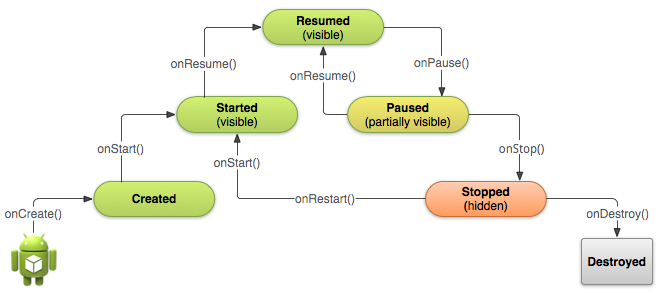
\includegraphics[scale=.5]{activity_state_machine.png}
\caption{The lifecycle of an Activity}
\label{fig:actlife}
\end{figure}

The states are
\begin{itemize}
	\item \textbf{Starting}. In the process of setting up.
	\item \textbf{Running}. In foreground.
	\item \textbf{Paused}. Not in foreground but active.
	\item \textbf{Stopped}. Inactive but remains in memory.
	\item \textbf{Destroyed}. Shut down and ready to be removed from memory.
\end{itemize}

There are multiple callback methods called when moving between states. We have already seen \texttt{onCreate} which is the only one that activities are required to override but there are several others.

\begin{itemize}
	\item \textbf{\texttt{onCreate()}}.\\
    \noindent This callback method is for the event of creating an activity and is called before the activity starts. It is typically used for initialization as we have been using it already.
	\item \textbf{\texttt{onStart()}}.\\
    \noindent Is called every time the activity starts, after entering the starting state. Here the activity becomes visible and prepares for entering the foreground and becoming interactive. This is where the app initializes the code that maintains the UI of the activity.
	\item \textbf{\texttt{onResume()}}.\\
    \noindent When entering the running state the activity is coming to the foreground and this callback is invoked. Here we should initialize components that are released by \texttt{onPause}, such as animations and camera.
	\item \textbf{\texttt{onPause()}}.\\
    \noindent This method is invoked when you are leaving your activity and it seizes to be in the foreground but is still visible. From there on it can either be resumed later or stopped. Here we must release system resources such as GPS and camera as well as animations but we should not perform long and heavy tasks of cleaning up here.
	\item \textbf{\texttt{onStop()}}.\\
    \noindent After your activity siezes to be visible, this callback is invoked. The \texttt{onPause} method is always called before this one and any large task of releasing resources should happen here. The activity is still in memory at this stage.
	\item \textbf{\texttt{onRestart()}}.\\
    \noindent If the activity goes from being stopped to starting it will invoke the \texttt{onRestart} method.
	\item \textbf{\texttt{onDestroy()}}.\\
    \noindent When you are removing your activity from memory this method is invoked but at what time exactly is unpredictable. To destroy our current activity we can call the \texttt{finish} method.
\end{itemize}

Using \texttt{Log.d} we can use printf debugging with certain tags and filter them with the Android Logcat as shown in figure \ref{fig:logfilt}. 

\begin{figure}[H]
\centering
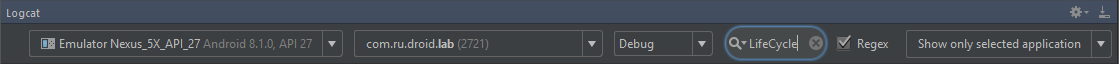
\includegraphics[scale=.6]{log.png}
\caption{Filter logs}
\label{fig:logfilt}
\end{figure}

Using \texttt{Log.d} we can monitor the lifecycle of the two activities found \href{https://github.com/JonSteinn/AndroidDevelopment/tree/master/examples/lab3/lifecycle}{here}. You should try various scenarios of navigating between the apps as well as rotating the screen and using the Android back button.

\subsection{Passing data between activities}
As we have already discussed, Intents are something of a bridge between activities. We use it to start a new activity but it can also be used to pass data between activities.

\begin{lstlisting}[style=A_Java]
Intent intent = new Intent(MainActivity.this, SecondActivity.class);
intent.put("SOME_KEY", "SOME_VALUE");
startActivity(intent);
\end{lstlisting}

The parameter we are using here is an instance of the current activity and a \texttt{.class} of the activity we want to lunch. This is called a reflection and is provides a way to get metadata on classes during runtime. The Intent constructor is overloaded so these are not the only options for parameters. We can use \texttt{getIntent()} to access the intent in the newly lunched activity and depending on the data type, there are various methods to access values given keys.

\begin{lstlisting}[style=A_Java]
Intent intent = getIntent();
String value = intent.getStringExtra("SOME_KEY");
\end{lstlisting}

In the provided example the first activity has a simple login UI with validation (using a simple hard coded map of accepted username and passwords) and if successful, we proceed to the next activity passing along the username for a personal greeting. The source code can be found \href{https://github.com/JonSteinn/AndroidDevelopment/tree/master/examples/lab3/login}{here} and a programming session \href{TODO}{here}.\\

We might also want to get data to other way around, from a lunched activity to the activity that lunched it. For that we can use \texttt{startActivityForResult} and the callback method \texttt{onActivityResult}. Suppose we have two activities A and B where A lunches B and expects results. Activity A must use a unique id to start the activity B for results and check if it matches when the callback is invoked. The activity B must set results before finishing which involves an intent of data and a result code (can be custom) which activity A can then check for.\\

The provided example shows an app where the main activity contains just a single button which upon clicking starts the second activity for result. In the second activity there is an input field and a button for sending back the result (the text in the input field) and then destroying itself. The main activity then uses a callback to set the text of its button with the value passed by the second activity, given that the id and code match. The source code can be found \href{https://github.com/JonSteinn/AndroidDevelopment/tree/master/examples/lab3/activityforresult}{here} and a programming session \href{TODO}{here}.

\subsection{Thread and activity memory issues}
TODO

\section{Layout inflater}
Before we look into fragments, we will take a look at another way of re-using code with layout inflaters. Suppose we want multiple repetition of the same partial layout on our screen like can be seen in figure \ref{fig:infldem}, it would be very tedious to write seperate views and code for all of them, especially if they become complicated.

\begin{figure}[H]
\centering
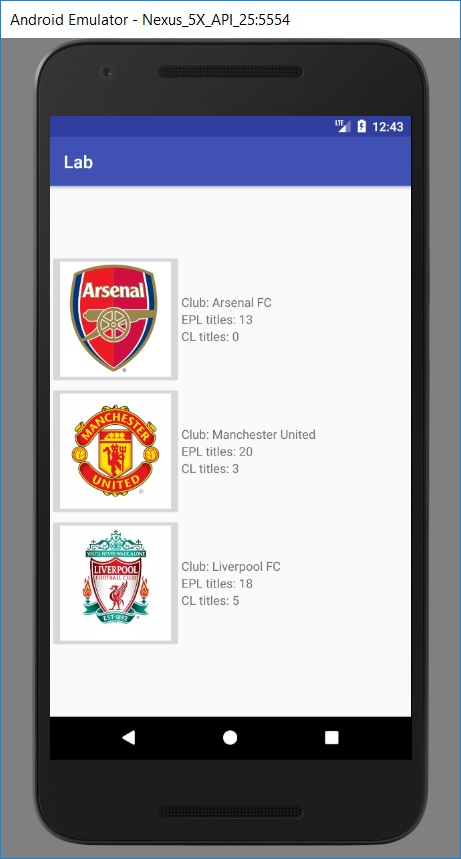
\includegraphics[scale=.5]{inflate_demo.png}
\caption{Same layout used 3 times with layout inflater}
\label{fig:infldem}
\end{figure}

To re-use a layout, we can use what is called a layout inflater. To do that we must create a new layout resource file with \menu{File > New > Android resource file} which can serve as a re-usable template. The provided example is the single team layout in figure \ref{fig:infldem}, used for each team. Note that all visible components of the UI are set in Java so without doing so, nothing would be visible. The figures are placec in the drawable resource folder and can be accessed directly in Java. Also note that we are not using \texttt{findViewById} from our instance (activity) but rather using the template view and searching for them within it. The source code for this example is available \href{https://github.com/JonSteinn/AndroidDevelopment/tree/master/examples/lab3/inflator}{here} and a programming session \href{TODO}{here}.

\section{Fragments}
Fragments are a re-usable UI component that can be added to an activity. They are similar to activities in many ways, something like a smaller version of activities. They have their own layout and lifecycle although their live depends on activities, that is their state depends on the state of their activity. The lifecycle of a fragment can be seen in figure \ref{fig:flife}.

\begin{figure}[H]
\centering
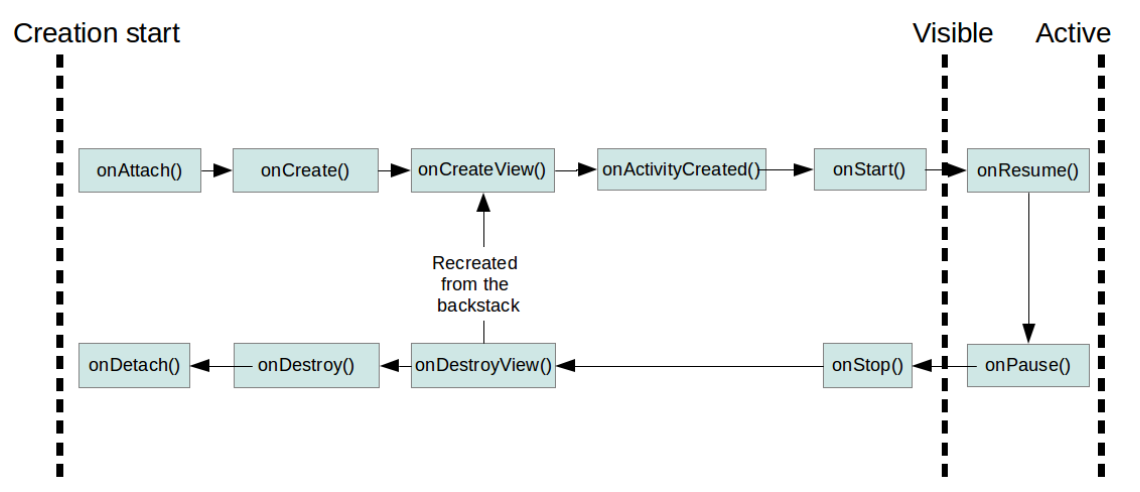
\includegraphics[scale=.75]{fragment_state_machine.png}
\caption{Fragment lifecycle}
\label{fig:flife}
\end{figure}

We will not go into much detail about the state or callbacks of a fragment. The \texttt{onCreateView} method must always be overwritten and it creates and returns the view hierarchy associated with the fragment. Another callback that we will have to use is \texttt{onActivityCreated} which is called when the parent activity has finished its own \texttt{onCreate} method.\\

Suppose we want to create a UI that is both suited for tablets or phones, or for both portrait and landscape mode on our phone. We could use a layout inflater or we could just remake the entire UI for both of them. We can also use fragments to create re-usable components that has all the logic and rendering for whatever we want to do, while the activity serves mostly as a container. An example of such a scenario can be seen in figure \ref{fig:freuse} where we have a list of something and upon clicking, it shows us more details on what was selected. Here we could have one activity that has two different layouts depending on the mode, one with two activities, each with its fragment and a navigation between the two while the other displays two fragments on the same activity and updates one from an event from the other.

\begin{figure}[H]
\centering
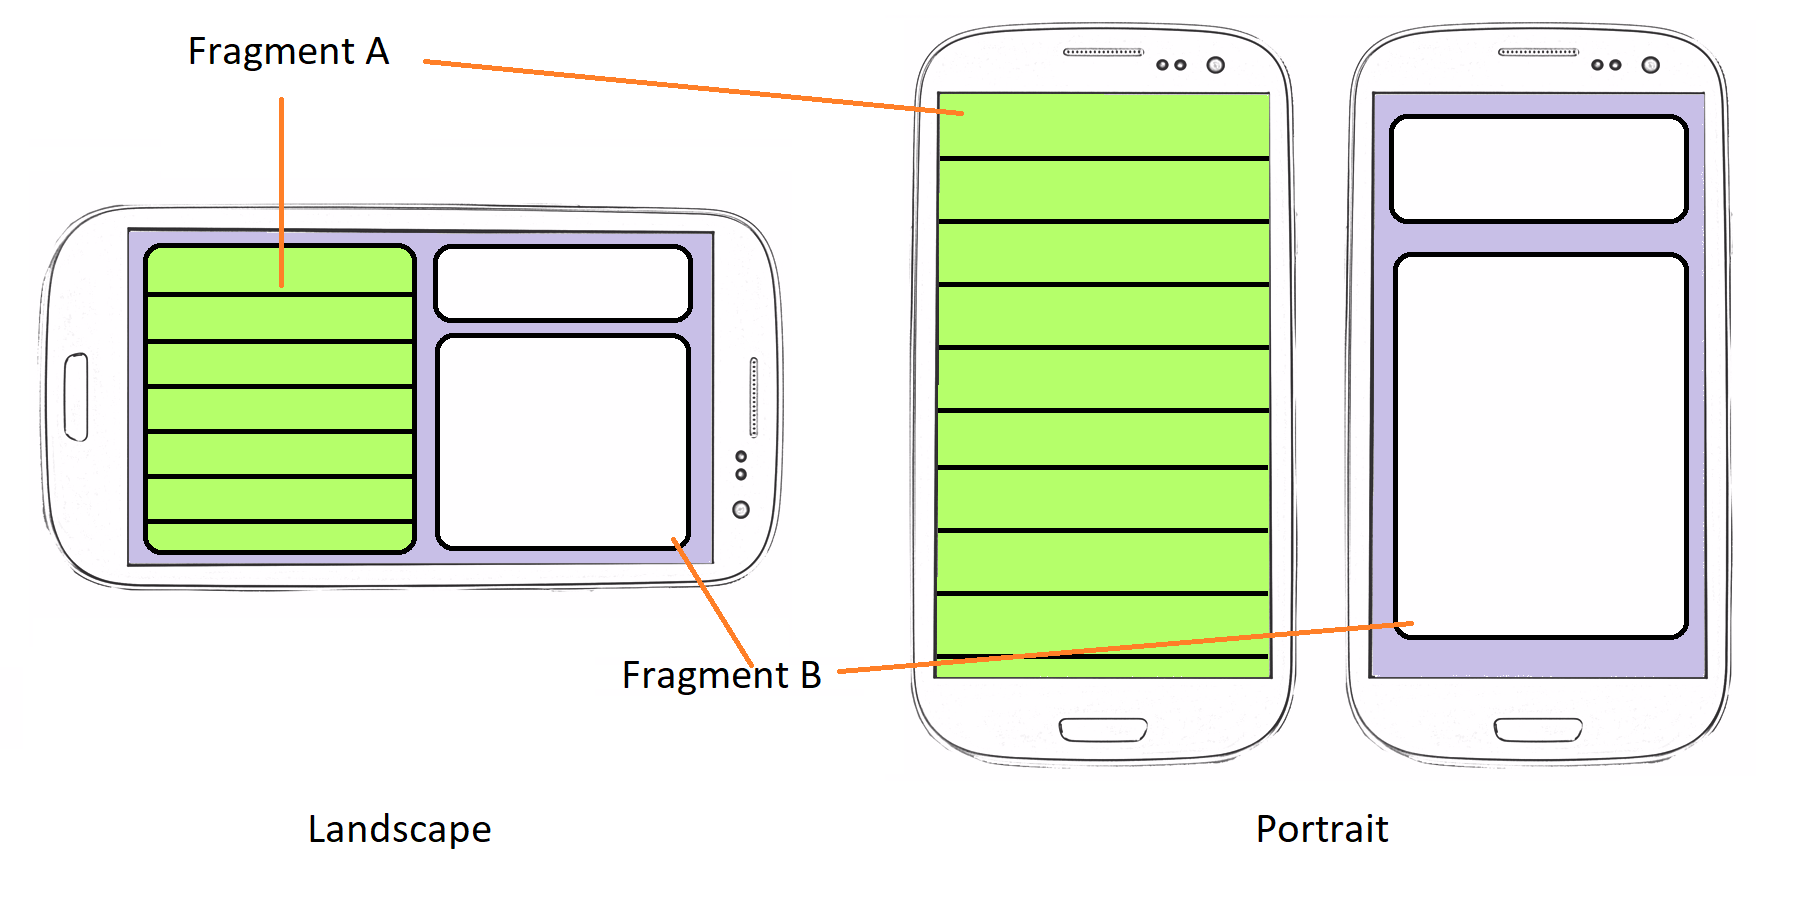
\includegraphics[scale=.4]{fragment_for_modes.png}
\caption{Re-usable fragments}
\label{fig:freuse}
\end{figure}

Lets start by creating a new resource file. Select layout as type, add orientation as a qualifier and set it to landscape and name the layout the same as your layout for your launcher activity. Android will automatically look for the landscape layout when it enters landscape mode. Next we want to create to new fragments, \menu{File > New > Fragment > Fragment (Blank)}. You do not need to include fragment factory methods or include interface callbacks.\\

In the provided example we create a simple app using fragments to support landscape and portrait mode. You can click on the box cover of a few video games and when you do you get a screenshot of the game in a new activity. If you however go to landscape mode and click a box cover, you get the screenshot on the same activity, to the other fragment's right. The sourcecode can be found \href{https://github.com/JonSteinn/AndroidDevelopment/tree/master/examples/lab3/fragments}{here} and the programming session \href{TODO}{here}.

\section{Assignment}
Your task is to implement a phonebook. It should be able to show a list of all persons, add a new person and view details on any specific person. You can use a hashmap as a fake database. The UI should be different for landscape and portrait mode. In landscape mode the menu should always be on the left side of the screen while in portrait you should swap between screens whenever you navigate. Figure \ref{fig:scetch} shows a prototype for the program you are expected to turn in. You are not required to use fragments.

\begin{figure}[H]
\centering
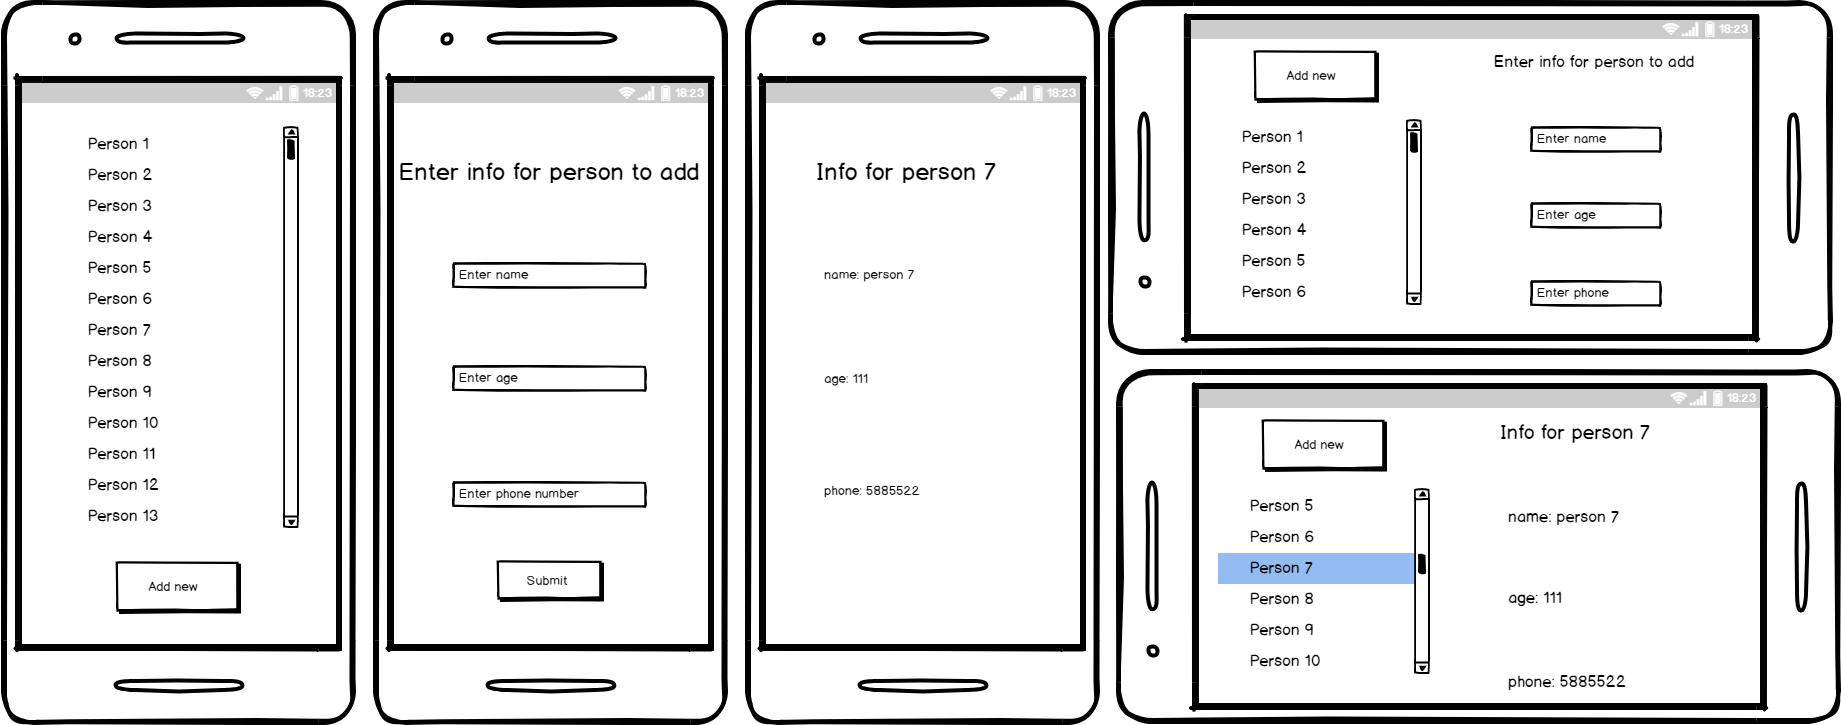
\includegraphics[scale=.2]{ui_scetch_for_assig.png}
\caption{A prototype of the assignment}
\label{fig:scetch}
\end{figure}